\documentclass[12pt,preprint]{aastex}

\usepackage{amsmath}

\begin{document}

\title{Something about Lens Models}

\author{First Author,\altaffilmark{1}
Second Author,\altaffilmark{2} and
Third Author\altaffilmark{3}}
\altaffiltext{1}{First place}
\altaffiltext{2}{Second place}
\altaffiltext{3}{Third place}

\begin{abstract}
This is an abstract.
\end{abstract}

\keywords{}

\section{Introduction}

See Figure \ref{fig:ASW0000kad}.

\appendix

\section{Essentials of Lensing Theory}



First we define comoving distances, as follows.
\begin{equation}
\int \frac{dz}{\sqrt{\Omega_m(1+z)^3 + \Omega_\Lambda}}
\end{equation}
\begin{equation}
\begin{aligned}
&D_S    &                                &\int_0^{a_S} \\
\noalign{\medskip}
&D_{LS} & = \frac c{H_0} \ \times \quad  &\int_{z_L}^{z_S} \\
\noalign{\medskip}
&D_L    &                                &\int_0^{z_L}
\end{aligned}
\end{equation}

Then define the arrival time, following \cite{1986ApJ...310..568B}.
Let $x,y$ be physical distances on the lens plane and $D_L$ be
comoving distances.  Then
\begin{equation}
l_{\rm geom} = \frac1{2D_L} \frac{D_S}{D_{LS}}
\left( (x-s_x)^2 + (y-s_y)^2 \right)
\end{equation}
\begin{equation}
\nabla^2 l_{\rm grav} = \frac{8\pi G}{c^2} \Sigma(x,y)
\end{equation}
But $l_{\rm grav}$ expands by $(1+z)$.

It is usual to work in terms of
\begin{equation}
\kappa = \frac{4\pi G}{c^2} \frac{D_L}{1+z} \frac{D_{LS}}{D_S} \Sigma
\end{equation}
known as the convergence.

The Laplacian $\nabla^2 f(x,y)$ is
\begin{equation}
 \frac{ f(x+\Delta x, y) + f(x-\Delta x, y) +
        f(x, y+\Delta y) + f(x, y-\Delta y) - 4 f(x,y) }
      {\Delta x \; \Delta y}
\end{equation}
in the limit of $\Delta x,\Delta y$ small.

\newpage

\bibliographystyle{apj}
\bibliography{ms}

\newpage

\begin{figure}
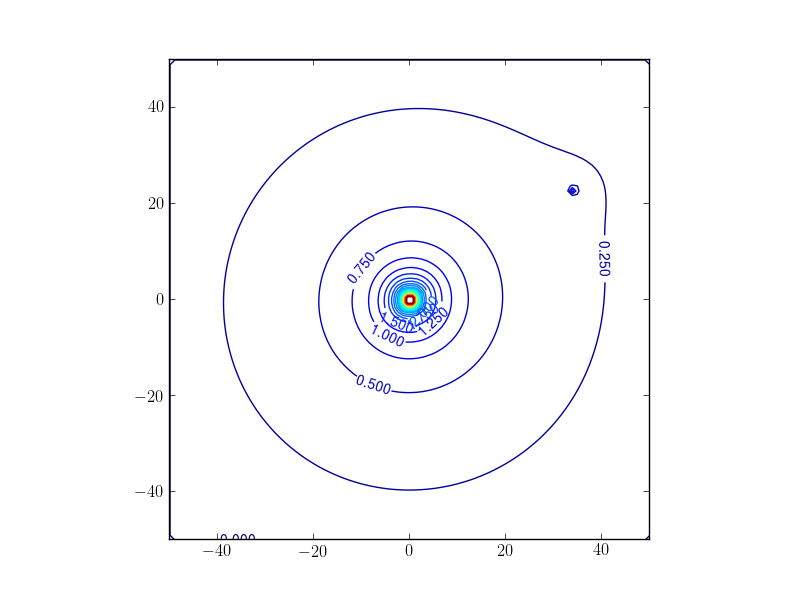
\includegraphics[width=.3\hsize]{ASW0000kadC_kappa.png}
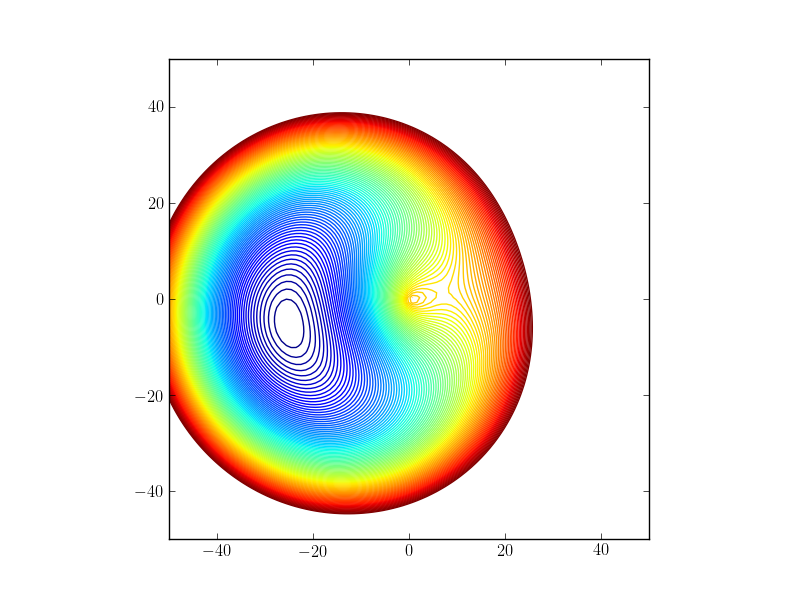
\includegraphics[width=.3\hsize]{ASW0000kadC_arriv.png}
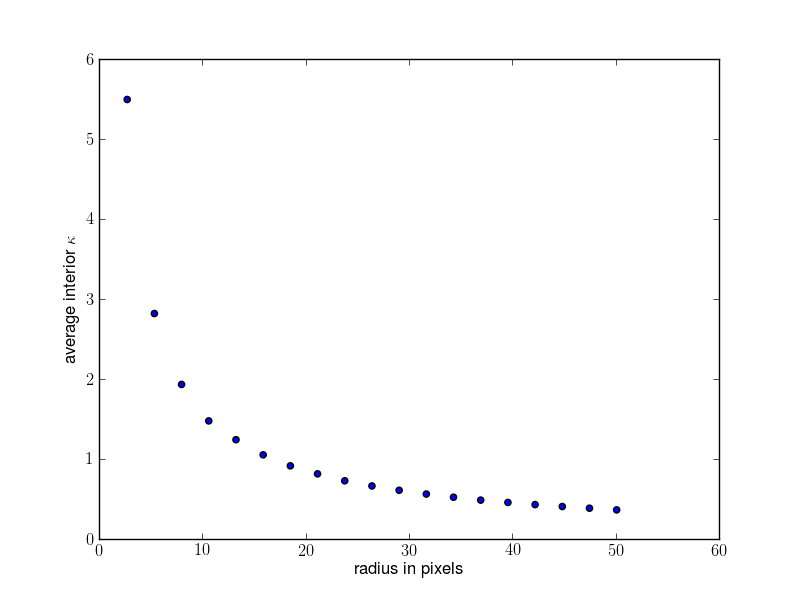
\includegraphics[width=.3\hsize]{ASW0000kadC_menc.png}
\caption{This is a figure.\label{fig:ASW0000kad}}
\end{figure}

\end{document}

